% vim: set spelllang=fr:
\chapter{Introduction}
\label{ch:intro}

\section{Objectifs}

\subsection{L'annotation en rôles sémantiques}

L'annotation en rôles sémantiques est une tâche d'analyse sémantique aux
applications nombreuses, telles que l'extraction et la recherche d'information,
la traduction automatique, ou encore le résumé automatique de textes.

Elle répond à la question « Qui a fait Quoi à Qui, Comment, Où et Quand ? ».
Prenons pour exemple la phrase \emph{Mrs. Aouda essaya vainement de retenir Mr.
Fogg} (extrait du \emph{Tour du monde en quatre-vingts jours} de Jules Verne).
En considérant pour exemple le cadre de FrameNet
(section~\ref{presentation_framenet}), une annotation en rôles sémantique du
prédicat \emph{essayer} déterminera que cette utilisation du verbe correspond à
une situation de tentative, puis identifiera parmi les syntagmes liés aux
verbes quel est l'Agent, l'Activité tentée, et le Résultat.  Ainsi, le résultat
de l'annotation serait :

\begin{figure}[ht]
    \centering
    \begin{tabular}{cccc}
    [Agent]  & \textbf{Tentative} & [Résultat]  & [Activité]         \tabularnewline
    Mrs. Aouda & \textbf{essaya}  & vainement & de retenir Mr. Fogg. \tabularnewline
    \end{tabular}
    \caption{\label{fig:introsrl}Le verbe \emph{essayer} déclenche la situation \emph{Tentative}.
    Les différents syntagmes liés au verbe jouent chacun un rôle sémantique.}
\end{figure}

Différentes informations sont disponibles après l'annotation en rôles
sémantiques :

\begin{itemize}
    \item Le prédicat ayant déclenché la frame est identifié. Dans la
        figure~\ref{fig:introsrl}, c'est un verbe, mais d'autres parties du
        discours peuvent déclencher une frame.
    \item La frame est identifiée, ici \emph{Tentative}.
    \item Enfin, les rôles exprimés sont annotés. Par exemple, \emph{Mrs.
        Aouda} est l'Agent.
\end{itemize}

\subsection{Applications}

% TODO est-ce que http://www.aclweb.org/anthology/D/D14/D14-1188.pdf
% est différent ou mieux que bazrafshan2013semantic ?
Selon \cite{gildea2002automatic}, l'annotation en rôles sémantiques est une
évolution naturelle de certains travaux sur l'extraction d'information où les
systèmes traitent des situations très spécifiques, par exemple la détection de
résultats d'évènements sportifs ou la détection dans des corpus journalistiques
de l'acquisition d'entreprises. En effet, à chaque nouveau système d'extraction
d'information dans un domaine différent, il est nécessaire de redéfinir les
différents patrons sémantiques et d'entraîner un nouveau système sur de
nouvelles données. En s'appuyant sur le corpus FrameNet et pour évoluer vers
une généralisation de ces systèmes, \cite{gildea2002automatic} présentent le
premier système général d'annotation en rôles sémantiques. Sans pour autant
remplacer les systèmes d'extraction d'information\footnote{TODO différences},
l'annotation en rôles sémantiques a été utilisée dans diverses applications,
notamment les systèmes de questions-réponses \citep{shen2007using},
l'extraction d'évènements \citep{exner2011using},  l'analyse d'opinions
\citep{das2012structure} ou la traduction automatique
\citep{bazrafshan2013semantic}. Un des intérêts de la généralité de
l'annotation en rôles sémantiques est de s'adapter facilement à de nouvelles
tâches. Ainsi, l'annotation en rôles sémantiques à été utilisée pour la
détection de plagiat \citep{osman2012improved}, la prédiction des cours de
bourse \citep{xie2013semantic}, la génération de scènes 3D
\citep{chang2014semantic}, ou l'interprétation de recettes de cuisine
\citep{malmaud2014cooking}.

\subsection{Contraintes}

% TODO 2014-10 intégrer à LIMA et le dire :)
Nous souhaitons que notre système d'annotation en rôles sémantiques puisse être
utilisé dans un environnement industriel dans lequel d'une part l'annotation en
rôles sémantiques fournit des informations utiles au développement des tâches
applicatives et d'autre part les domaines à couvrir ne sont pas connus à
l'avance. Les contraintes suivantes découlent de ces prérequis.

\paragraph{Cadre ouvert} Se contenter de certaines situations dans un domaine
fermé n'est pas satisfaisant. Les inventaires de sens utilisés doivent couvrir
au maximum les différents sens des mots d'une langue.

\paragraph{Langue française} Le français dispose d'un nombre limité de
ressources sémantiques en cadre ouvert. Il n'existe pas aujourd'hui de VerbNet
(section~\ref{presentation_verbnet}), WordNet
(section~\ref{presentation_wordnet}) ou de FrameNet
(section~\ref{presentation_framenet}) du français avec une couverture et une
qualité proches de leurs équivalents respectifs en langue anglaise. Ne
disposant pas des moyens pour créer de telles ressources manuellement, le
système présenté doit pouvoir se contenter de transpositions automatiques de
ces ressources vers le français. Avec cette approche de mutualisation des
ressources au niveau de la langue, chaque nouvelle utilisation d'une de nos
ressources est l'occasion de l'améliorer à la fois pour utilisation immédiate
mais aussi pour les utilisations futures.

\paragraph{Simplicité} Nous voulons que notre système soit très simple à mettre
en place et qu'il soit tout aussi facile de corriger quelques erreurs
spécifiques, même au prix d'une performance moins bonne que des approches plus
complexes dans le cas général. La stratégie que nous adoptons est de simplifier
nos systèmes, et des les améliorer une fois qu'ils ont montré leurs limites.

\paragraph{Efficacité} Cette contrainte est moins forte que les autres, mais
reste nécessaire pour que les solutions présentées puissent être utilisées à
large échelle. L'annotation en rôles sémantiques est un problème difficile de
classification automatique et certains systèmes ont des temps d'entraînement et
d'exécution trop longs pour l'utilisation que nous voulons en faire ici.

\paragraph{Libre diffusion} Enfin, il est important que les outils et
ressources soient au maximum libre d'accès afin que d'autres puissent les
utiliser et les étudier. Pour cette raison, une grande partie du code source
écrit pendant cette thèse est disponible sur GitHub.

% MEGATODO faire que ce soit le cas
Ces contraintes seront utilisées pour évaluer à la fois l'état de l'art et les
approches présentées.

\subsection{Moyens}
\label{objectifs_these}

% TAL a besoin d'infos sur les verbes, c'est difficile et fragile, et on a
% besoin d'énormes corpus, donc on essaie les lexiques
Le Traitement Automatique des Langues requiert des lexiques et de larges
quantités de données annotées pour analyser efficacement des textes dans le
domaine général. Obtenir cette quantité de données est un problème en soi connu
sous le nom de "knowledge acquisition bottleneck" en désambiguïsation lexicale
\citep{gale1992method,navigli2009word}. Le problème se pose aussi pour
l'annotation en rôles sémantiques où la quantité de données annotées est
limitée \citep[section 1]{das2012structure}. Il est possible de résoudre ce problème
domaine par domaine en annotant de grandes quantités de données pour chaque
domaine, mais d'autres stratégies sont nécessaires pour atteindre nos objectifs
dans un grand nombre de domaines. Une possibilité est d'utiliser au mieux les
données annotées en perfectionnant les algorithmes existants, une autre est
d'utiliser intelligemment les données non annotées qui existent en quantité
bien plus importante. Une troisième possibilité, celle que nous choisissons
d'explorer ici, est d'exploiter des lexiques couvrant l'interface
syntaxe-sémantique sur une large partie du vocabulaire. C'est ce qui est fait
par exemple dans VerbNet où les traits partagés par les mêmes verbes sont
explicitement notés, ce qui permet à chaque modification dans VerbNet
d'améliorer le traitement de plusieurs verbes au lieu d'un seul.

% VerbNet a montré son efficacité dans le domaine de par son approche
% pragmatique. Vient des classes de Levin, donne des correspondances entre
% syntaxe et sémantique
Deux difficultés majeures qu'affrontent les créateurs de lexique sont la
granularité de sens et la distinction des sens. Ces deux difficultés sont
gérées par les classes de Levin \citep{levin1993english}. Dans ces classes, les
verbes sont classifiés principalement à travers leur alternances syntaxiques,
ce qui fournit un critère qui est à la fois facilement observable et qui
produit des distinctions sémantiques intéressantes. VerbNet
\citep{kipperschuler2005verbnet} est un lexique électronique basé sur les
classes de Levin. Il encode non plus les alternances mais les cadres de
sous-catégorisation valables pour chaque classe, et rajoute des informations de
rôle et de sémantique à travers une logique des prédicats simplifiée. De
nouvelles classes, constructions et verbes ont étés ajoutés à VerbNet au fil
des ans. Au-delà de son encodage efficace, VerbNet est un lexique adapté à la
tâche d'annotation en rôles sémantiques : on peut utiliser un cadre de
sous-catégorisation pour associer des syntagmes à des rôles thématiques
\citep{swier2005exploiting,pradet2013revisiting}. Grâce à sa couverture élevée
(plus de quatre mille verbes distincts) et son groupement de verbes utile,
VerbNet est bien adapté à l'annotation en rôles sémantiques.

% De la même manière, WordNet est complémentaire à VerbNet
WordNet est une autre ressource qui complète VerbNet en nous fournissant des
informations sur le sens des verbes inclus dans VerbNet grâce au projet
SemLink, mais aussi sur le sens des mots liés au verbe, ce qui permet de

\begin{itemize}

    \item désambiguïser la classe VerbNet utilisée,

    \item et de respecter les restrictions de sélections indiquées par VerbNet pour
        le sujet et les objets du verbe.

\end{itemize}


% Dans les langues autres que l'anglais, cette ressource utile n'existe pas
% mais ne demande qu'à exister étant donné le potentiel \textit{cross-lingual}
% de VerbNet. Il y a souvent des ressources proches, moins utiles, plus
% linguistiques, existent.
Cependant, un VerbNet et un WordNet de qualité n'existent pour le moment que
pour l'anglais. De telles ressources seraient pourtant encore plus utiles pour
les langues moins dotées où les corpus annotés en rôles sémantiques n'existent
pas. VerbNet a un potentiel inter-linguistique, visible notamment avec le
portuguais \citep[section 2.2.2]{kipperschuler2005verbnet}. Adapter VerbNet
vers une nouvelle langue suffisamment proche de l'anglais permet de conserver
sa structure, ainsi que l'information sémantique et les rôles thématiques, ce
qui donne la possibilité de produire un lexique utile sans des années de
travail manuel.

% TODO étendre, mais comment ? Inclure méthodes et ressources plus haut ?
Une fois que ces ressources ont été traduites vers le français, il faut les
utiliser pour réaliser la tâche d'annotation en rôles sémantiques.

Cette thèse fournit donc les \emph{ressources} nécessaires en traduisant
WordNet et VerbNet (Partie~\ref{part:translation}) et les \emph{méthodes}
(Partie~\ref{part:srl}) répondant à ces objectifs.

\section{Ressources lexicales utilisées}

La première ressource lexicale à tirer parti de la possibilité de représenter
le lexique sous la forme d'un graphe est WordNet \citep{fellbaum1998wordnet}.

\subsection{WordNet}
\label{presentation_wordnet}

L'élaboration de WordNet a commencé en 1985 \citep{miller1990introduction}.
Établi sur des principes psycholinguistiques, WordNet propose quatre graphes
pour les quatre parties du discours formant une classe ouverte : noms, verbes,
adjectifs, adverbes. Les nœuds du graphe sont des ensembles de synonymes
(\emph{synonym sets} ou \emph{synsets}). Un synset regroupe plusieurs mots, une
définition, et potentiellement des exemples.

% TODO placement des figures une fois le texte un peu plus stable

\begin{figure}[t]
    \centering
    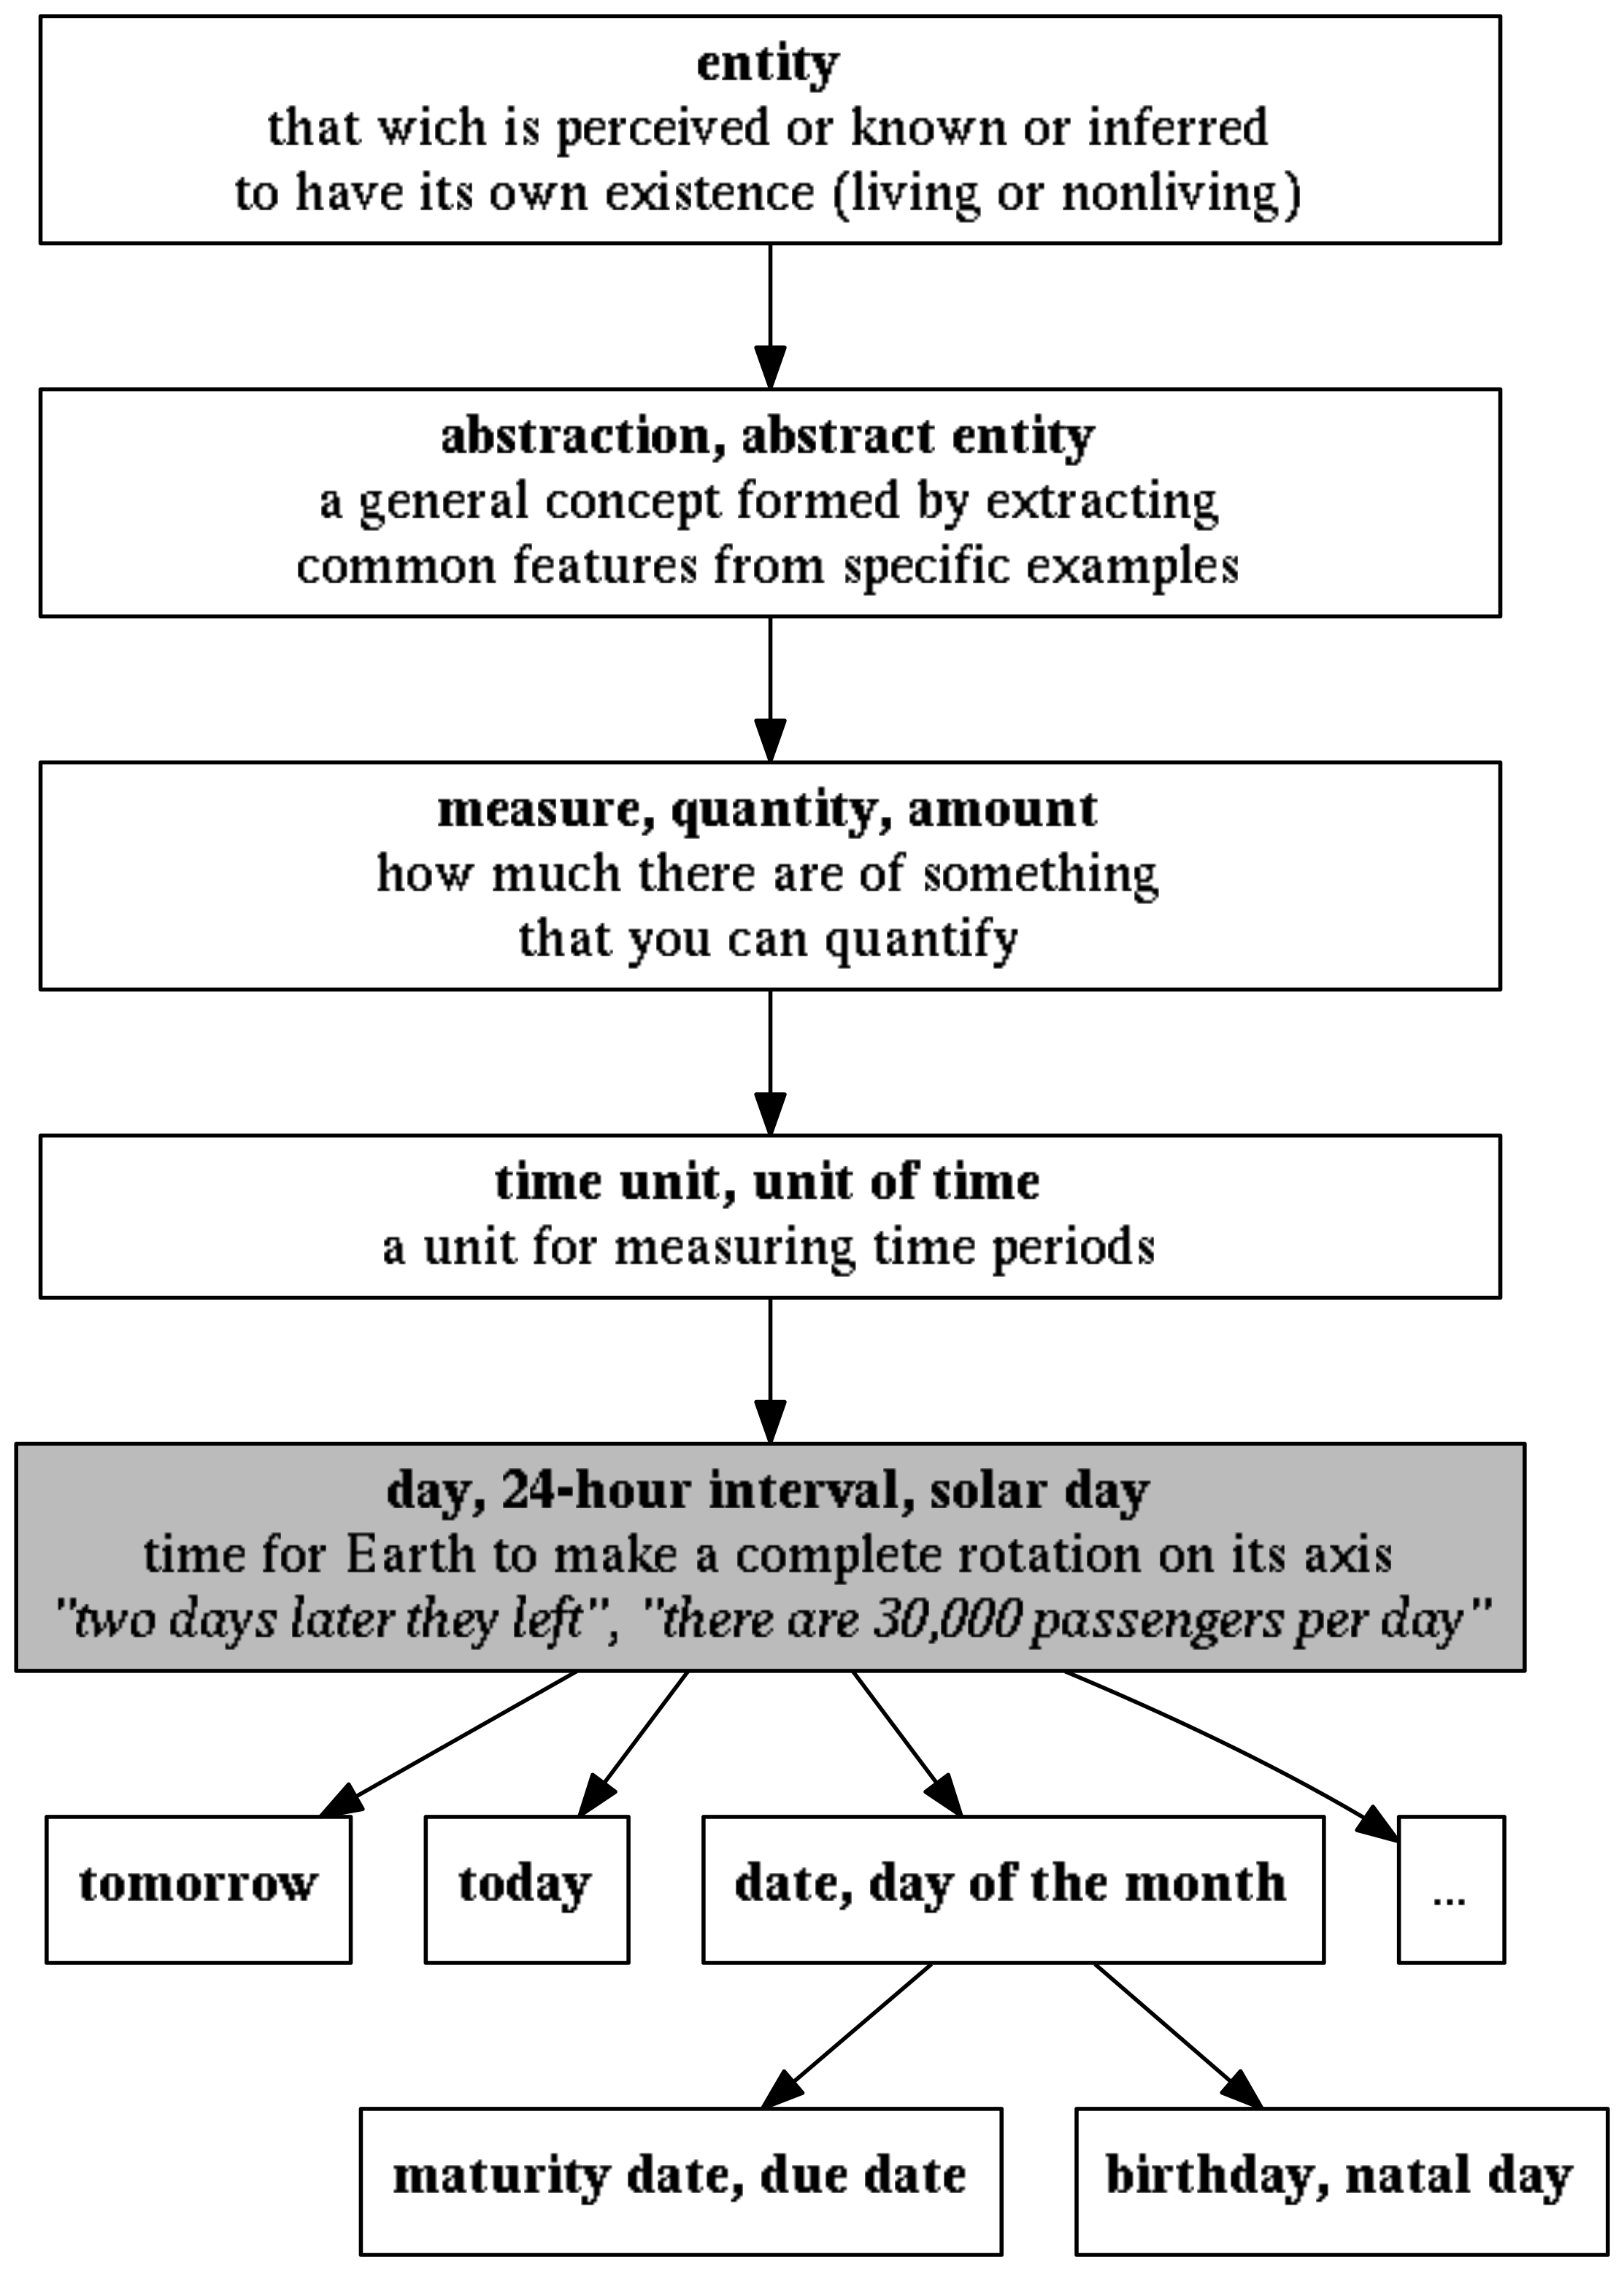
\includegraphics[width=0.6\textwidth]{fig/wordnet_hypernymy.png}
    \caption{\label{fig:wordnet_hypernymy}Hypéronymie dans WordNet autour du
        synset \emph{day}. Les synsets au-dessus de \emph{day} sont ses hypéronymes
        (\emph{day} est-un \emph{time unit}), et les synsets au-dessus font partie de
        ses hyponymes (\emph{tomorrow} est-un \emph{day}).}
\end{figure}

Chaque synset est lié à d'autres synsets à travers un certain nombre de
relations telles que l'hypéronymie, la méronymie de partie (\emph{guidon} est
un méronyme de partie de \emph{vélo}), l'antonymie, etc. Si on ne considère que
l'hypéronymie, WordNet peut être visualisé comme un arbre
(Figure~\ref{fig:wordnet_hypernymy}). En considérant les autres relations,
WordNet est un graphe (Figure~\ref{fig:wordnet_relations}).

\begin{figure}[t]
    \centering
    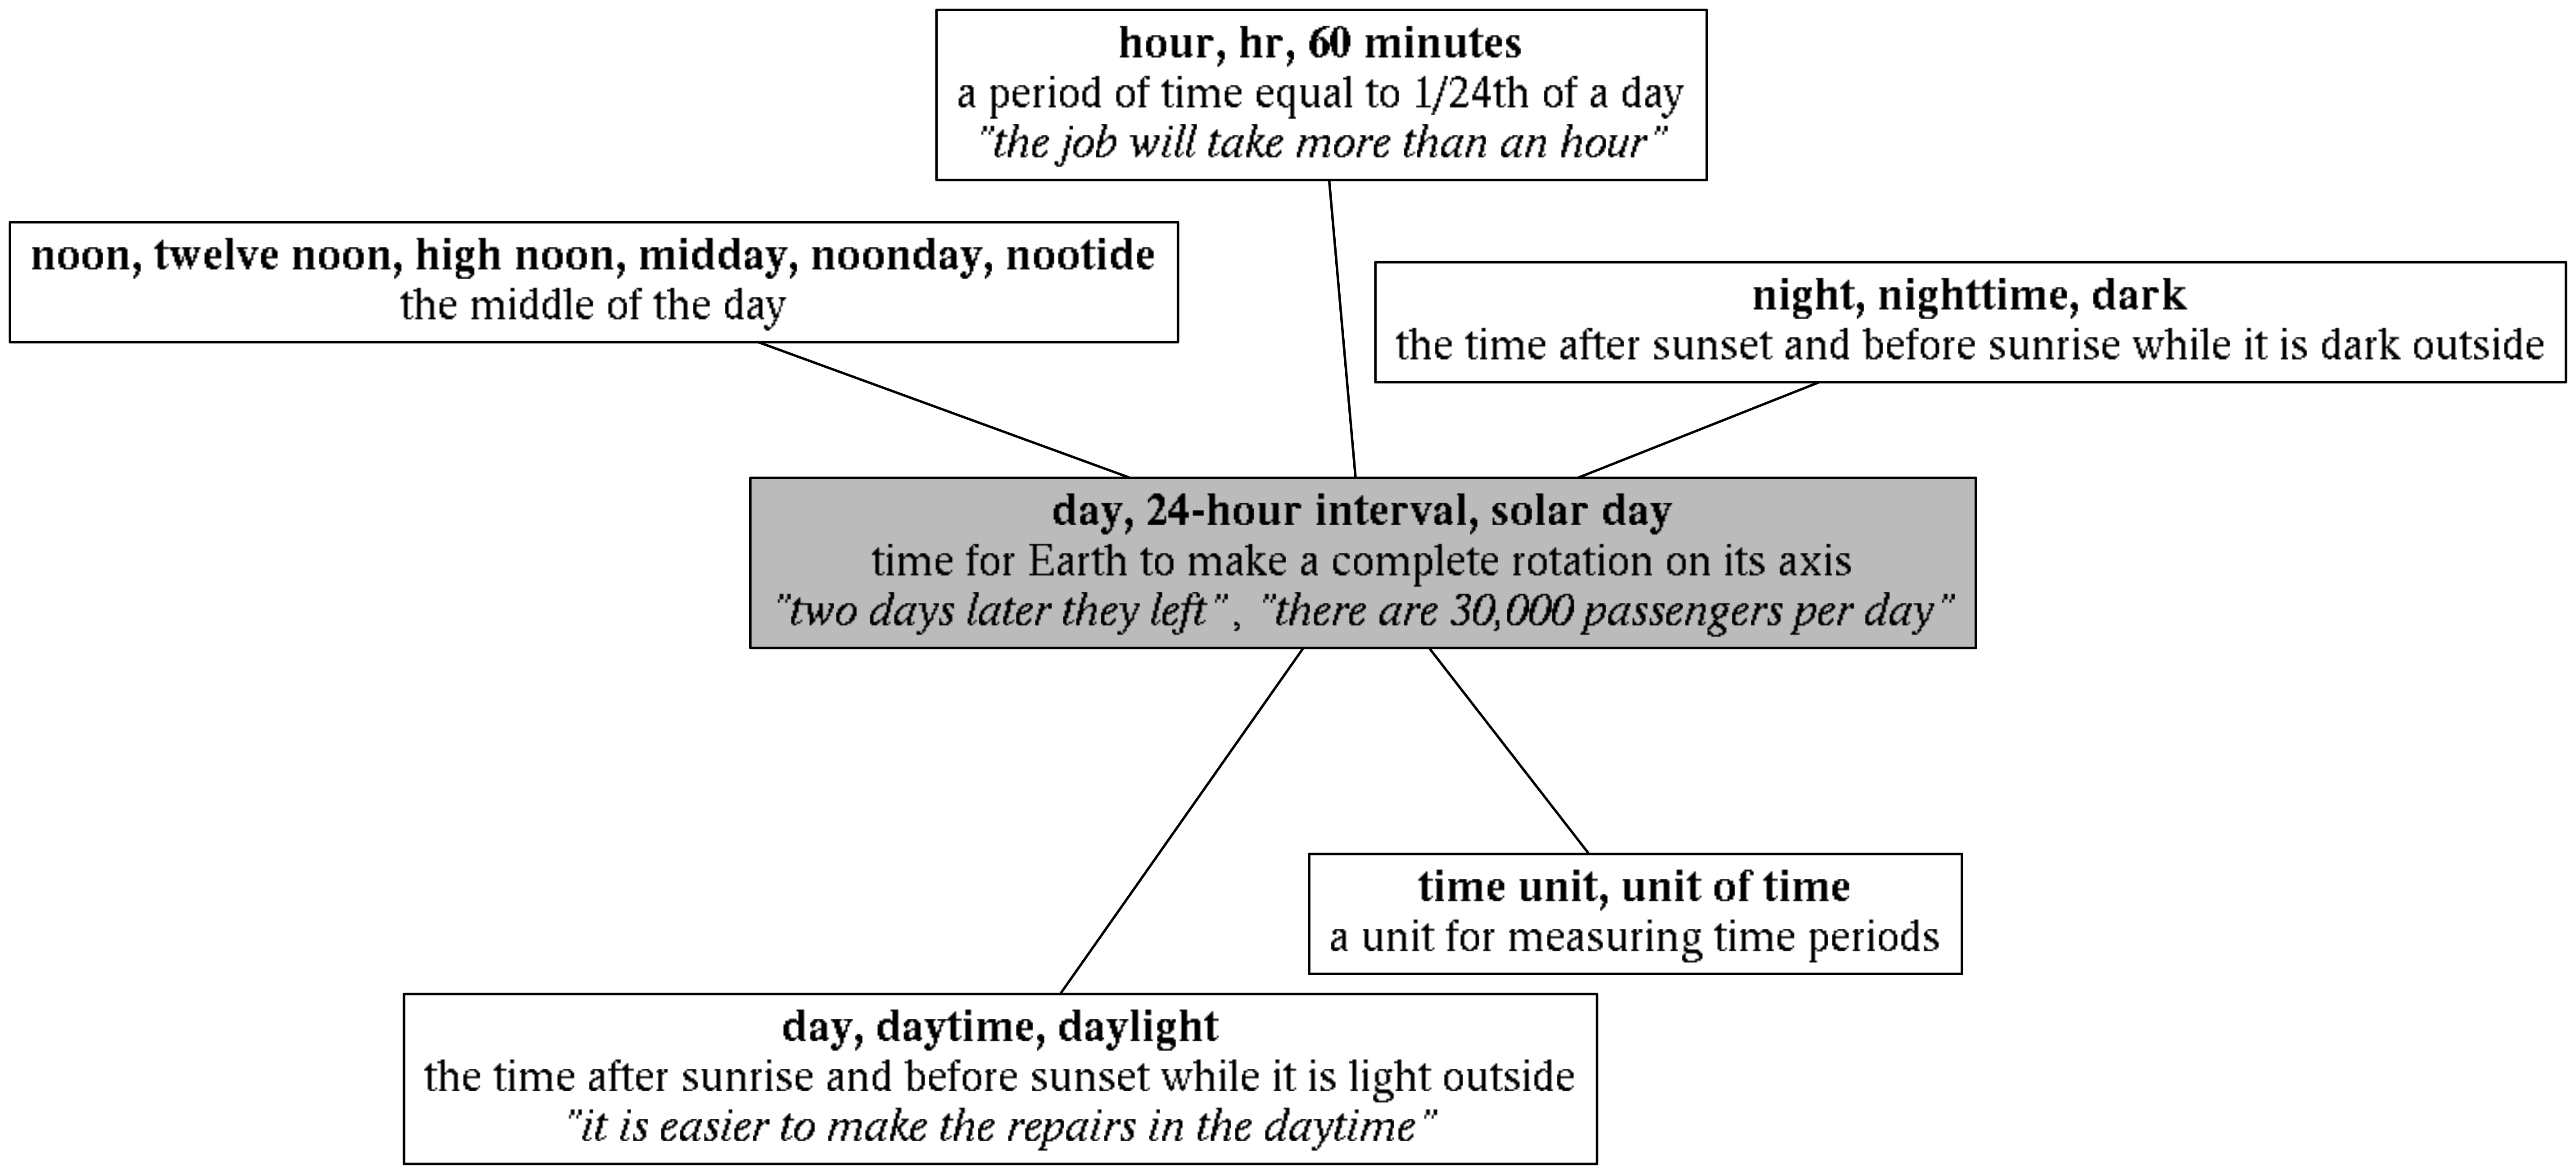
\includegraphics[width=0.7\textwidth]{fig/wordnet_relations.png}
    \caption{\label{fig:wordnet_relations} Le synset \emph{day} est aussi lié à
        d'autres synsets si on considère d'autres relations que l'hypéronymie et
        l'hyponymie.}
\end{figure}

Les sens proposés ont étés utilisés pour annoter différents corpus
\citep{petrolito2014survey}, ce qui a permis d'entraîner des systèmes
supervisés. WordNet est rapidement devenu le standard de la désambiguïsation
lexicale et a été utilisé dans de nombreuses campagnes d'évaluation
\citep{navigli2009word}. C'est aussi une ressource très utilisée de manière
générale \footnote{Au moment de l'écriture de ce manuscrit, ses 10~000
    citations sur Google Scholar sont le meilleur moyen de l'attester.}.

\subsection{Les classes de Levin}

Les classes de Levin \citep{levin1993english} sont une classification des
verbes anglais établie suivant un principe simple : le comportement syntaxique
des verbes détermine en partie leur sens. Après avoir défini un certain nombre
d'alternances de diathèses possibles, les verbes sont classés en groupes
partageant les mêmes alternances.

Par exemple, les \emph{fill verbs} tels que \emph{staff}, \emph{coat} ou encore
\emph{pollute} acceptent notamment la \emph{locatum subject alternation} :

\begin{itemize}
    \item Leslie staffed the store with employees
    \item The employees staffed the store
\end{itemize}

mais n'acceptent pas par exemple, la \emph{conative alternation} :

\begin{itemize}
    \item ~ \emph{Leslie staffed the store with employees}
    \item * \emph{The store staffed with employees}
\end{itemize}

Ainsi, pour chaque groupe de verbes, différents critères précis permettent de
distinguer ces verbes d'autres qui n'ont pas les mêmes propriétés.

Cette classification a trois intérêts pour l'annotation en rôles sémantiques :

\begin{itemize}

    \item Une grande majorité des verbes anglais sont couverts, rendant la
        ressource utile pour des annotations à large échelle.

    \item La classification est hiérarchique et regroupe de nombreux verbes :
        avec une cinquantaine de classes principales, des généralisations et
        partages d'informations entre les verbes de classes identiques ou
        proches sont possibles.

    \item Les comportements syntaxiques déterminent les comportements
        sémantiques, ce qui correspond au schéma classique de l'annotation en
        rôles sémantiques qui s'appuie sur une analyse syntaxique.

\end{itemize}

%\subsection{Intersection des classes de Levin}

% TODO raccourcir sans dire de bêtises

Dans les classes de Levin, toute distinction de classe doit s'appuyer sur un
critère clairement observable, tel que le comportement syntaxique ou les
propriétés morphologiques d'un verbe. Et ceci même si la distinction entre deux
classes est motivée par la volonté de prendre en compte une différence
sémantique entre deux groupes de verbes.

Pour cette raison, les groupements de verbes sont parfois grossiers d'un point
de vue sémantique. Ainsi, dans les \textit{put verbs} se trouve la classe
\textit{Pocket} qui regroupe les verbes "mettre dans sa poche" (\emph{put}) et
"mettre en prison" (\emph{jail}). Cependant, le comportement syntaxique est le
même : le regroupement est logique et les différences de sens ne sont a priori
pas gênantes pour des tâches telles que l'annotation en rôles sémantiques qui
ne se basent pas sur le sens précis des verbes. Il est possible d'affiner
automatiquement les classes de Levin en réalisant des intersections de classes
: les verbes obtenus seront alors définis plus strictement
\citep{dang1998investigating}. Cette possibilité n'est cependant pas utilisée
dans nos travaux.

\subsection{VerbNet}
\label{presentation_verbnet}

VerbNet \citep{kipperschuler2005verbnet} est une version électronique des
classes de Levin qui ont été améliorées sur plusieurs fronts avec :

\begin{itemize}

    \item de nouvelles classes provenant de \cite{korhonen2004extended}
        intégrant les verbes acceptant des complétives, mais aussi des
        syntagmes adjectivaux et adverbiaux ou encore des particules,

    \item de nouveaux verbes provenant de \cite{dorr2001lcs},

    \item la liaisons des verbes à WordNet, OntoNotes, PropBank et FrameNet
        dans le cadre du projet SemLink \citep{palmer2009semlink}

    \item de nombreuses corrections au fil des versions, une des améliorations
        prévues dans le futur étant d'ajouter d'autres verbes via l'étude de
        large corpus \citep{bonial2013expanding}.

\end{itemize}

Ces améliorations ont à la fois contribué à VerbNet en largeur (nouvelles
classes) et en profondeur (nouveaux verbes, nouvelles constructions
syntaxiques). La base de données continue d'évoluer, la dernière version au
moment de l'écriture de ce manuscrit étant la 3.2. Malheureusement, la version
3.2 évolue sans que soient marqués clairement les sous-versions : suivant le
jour de téléchargement de VerbNet, nous pouvons avoir à disposition la version
3.2.1, 3.2.2 ou 3.2.3, sans pouvoir clairement distinguer ces trois versions.
Pour cette raison, nous rendons disponibles la version 3.2 de VerbNet datant
d'avril 2013 que nous utilisons dans l'ensemble de ce travail à l'adresse
suivante : \url{https://github.com/pquentin/verbnet/archive/v3.2_2013-04.zip}.

% TODO mieux décrire la hiérarchie et ses niveaux
VerbNet contient 3769 lemmes, 5257 entrées réparties en 500 sous-classes dont
270 classes de niveau 2 et 109 classes de niveau 1. La hiérarchie est
relativement plate. Pour chaque classe, ce lexique indique :

\begin{itemize}
        \item la liste des verbes de la classe,
        \item les rôles thématiques en jeu ainsi que leur restrictions de sélection,
        \item la liste des \emph{frames} VerbNet.
\end{itemize}

Une frame inclut une phrase d'exemple, une formule syntaxique donnant la
liaison entre les syntagmes et les rôles thématiques, une formule sémantique
basée sur la logique des prédicats explicitant la relation entre les
participants et les évènements.

% TODO exemple

% TODO autre exemple non intuitif avec verbe complet en bas

% TODO Introduire fig:example_srl
 VerbNet a montré la cohérence de sa classification et est très
utilisé, notamment pour l'annotation en rôles sémantiques
\citep{swier2005exploiting,palmer2013semantic} où il présente l'intérêt de ne
pas être restreint à un domaine spécifique tout en couvrant une large partie
des occurrences des verbes anglais dans un texte donné.

\begin{figure}[ht]
    \centering
    \begin{tabular}{ccc}
        \toprule
        Carol & crushed   & the ice \\
        Agent & V         & Patient \\
        \midrule
        The ice & crushes & easily  \\
        Patient & V       &         \\
        \bottomrule
    \end{tabular}

    \caption{\label{fig:example_srl}Ces deux phrases annotées avec la classe
    VerbNet \texttt{carve-21.2} montrent que la position des arguments ne
détermine pas à elle seule les rôles sémantique. Ici, le sujet syntaxique
correspond d'abord à l'Agent puis au Patient.}

\end{figure}


\subsection{Les Verbes Français et Lexique-Grammaire}

% TODO mieux structurer : avantage *puis* inconvénient (ou l'inverse)
À partir des années 70 deux ressources lexicales pour les verbes français ont
été dévelopées : LVF et LG\footnote{Plus tard, dans les années 1990, une autre
    ressource a été dévelopée : Dicovalence. Nous ne l'utilisons presque pas
dans nos travaux.}. Pourquoi ne pas utiliser ces ressources directement ?  Un
des intérêts des classes de Levin et de VerbNet par rapport aux ressources
françaises est leur approche pragmatique qui se traduit notamment par l'absence
de prise en compte des emplois métaphorique d'un verbe donné. Ainsi, LG inclut
des usages tels que \textit{Il galopait dans son esprit que Marie allait venir}
qui peuvent induire en erreur une application.  Certains usages métaphoriques
peuvent certes être prise en compte dans VerbNet, mais ils n'y sont pas par
défaut. En effet, \cite{brown2012semantic} proposent une analyse systématique
des emplois métaphorique de deux verbes représentatifs et montrent qu'utiliser
VerbNet pour raisonner sur les emplois métaphorique d'un texte est en partie
possible au prix d'une complexité plus importante et de prédicats sémantiques
moins précis.

LVF (Les Verbes Français, \cite{dubois1997verbes}) contient environ 25000
entrées classées en quatre niveaux :

\begin{itemize}

    \item 14 classes génériques (par exemple \emph{E : Verbes de mouvement}),

    \item 54 sous-classes sémantico-syntaxiques (par exemple \emph{C1 :
        s'exprimer par un son, une parole}),

    \item 246 sous-classes syntaxiques (par exemple \emph{M3b : imprimer tel
        mouvement à quelquec chose} et

    \item 533 sous-types (par exemple \emph{R3b.2 : défaire l'opération
        faite}).

\end{itemize}

% TODO exemple

LG (Lexique-Grammaire, \cite{gross1975methodes,boons1976structure}) comporte
lui 14 000 entrées classifiées en 67 «~tables~», chaque table groupant des
verbes partageant la même propriété définitoire syntaxique et potentiellement
une sémantique similaire. Chaque colonne de la table encode des restrictions
supplémentaires s'appliquant à certains des verbes de la table.

% TODO exemple


Les classes LVF et les tables LG peuvent toutes les deux être comparées aux
classes VerbNet. Cependant, ces ressources n'encodent ni les rôles thématiques
ni les formules sémantiques \footnote{Les notions de rôles thématiques et
d'évènement n'étaient pas répandues dans les années 1970.}.  C'est la raison
principale pour laquelle nous voulons construire une nouvelle ressource
française, \verbenet{} (Chapitre~\ref{ch:verbnet}). Cette ressource tire profit
d'une part des ressources existantes pour le français avec un encodage
sémantique et syntaxique riche, et d'autre part de l'information sémantique
présente dans VerbNet pour l'anglais, une langue proche du français.

\section*{Conclusion}

Après avoir introduit le cadre de nos travaux et présenté les différentes
ressources que nous utilisons, le chapitre suivant présente l'état de l'art qui
est le socle sur lequel nos travaux s'appuient.
